\documentclass{standalone}
\usepackage[utf8]{inputenc}
\usepackage[T1]{fontenc}
\usepackage{graphicx}
\usepackage{amsmath}
\usepackage[american,siunitx]{circuitikz}
\usetikzlibrary{arrows,shapes,calc,positioning}



    
\begin{document}
  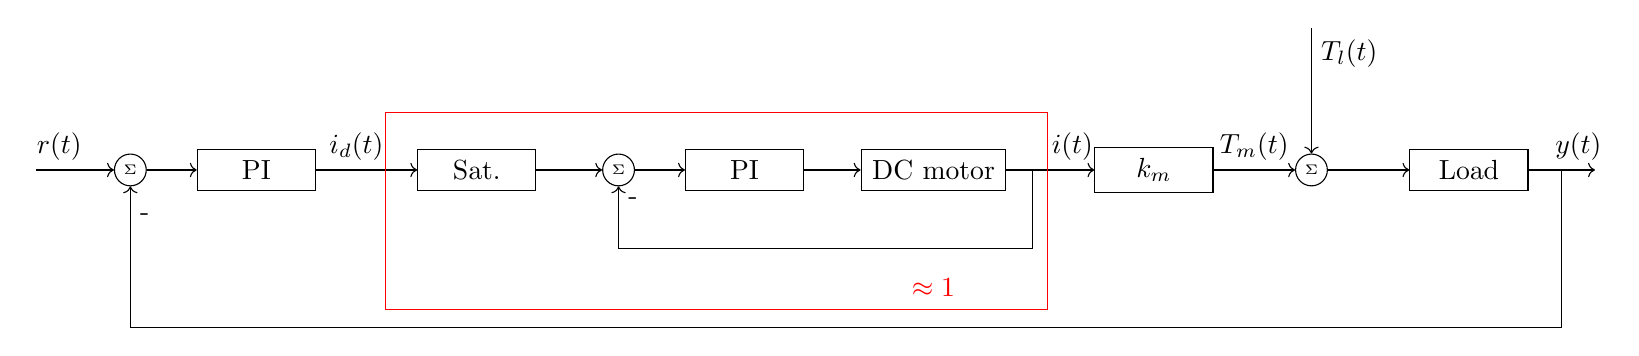
\begin{tikzpicture}[node distance=22mm, block/.style={rectangle, draw, minimum width=15mm, inner sep=4pt}, sumnode/.style={circle, draw, inner sep=2pt}]
    
    \node[coordinate] (input) {};
    \node[sumnode, right of=input, node distance=12mm] (sumerr) {\tiny $\Sigma$};
    \node[block, right of=sumerr, node distance=16mm] (f2)  {PI};
    \node[block, right of=f2, node distance=28mm] (sat)  {Sat.};
    \node[sumnode, right of=sat, node distance=18mm] (sumerr1) {\tiny $\Sigma$};
    \node[block, right of=sumerr1, node distance=16mm] (f1)  {PI};
    \node[block, right of=f1, node distance=24mm] (plant1)  {DC motor};
    \node[block, right of=plant1, node distance=28mm] (km)  {$k_m$};
    \node[sumnode, right of=km, node distance=20mm] (sumdist) {\tiny $\Sigma$};
    \node[block, right of=sumdist, node distance=20mm] (plant2)  {Load};
    \node[coordinate, above of=sumdist, node distance=18mm] (dist2)  {};

    \node[coordinate, right of=plant2, node distance=16mm] (output) {};

    \draw[->] (input) -- node[above, pos=0.3] {$r(t)$} (sumerr);
    \draw[->] (sumerr) -- node[above] {} (f2);
    \draw[->] (f2) -- node[above, pos=0.4] {$i_{d}(t)$} (sat);
    \draw[->] (sat) -- node[above] {} (sumerr1);
    \draw[->] (sumerr1) -- node[above] {} (f1);
    \draw[->] (f1) -- node[above] {} (plant1);
    \draw[->] (plant1) -- node[coordinate,pos=0.3] (meas1)  {} node[above, near end] {$i(t)$} (km);
    \draw[->] (km) -- node[above] {$T_m(t)$} (sumdist);
    \draw[->] (meas1) -- ++ (0,-10mm) -| node[right, pos=0.9] {-} (sumerr1);
    \draw[->] (sumdist) -- node[above, near end] {} (plant2);
    \draw[->] (plant2) -- node[coordinate] (meas) {} node[above, near end] {$y(t)$} (output);
    \draw[->] (dist2) -- node[right, pos=0.2] {$T_l(t)$} (sumdist);
    \draw[->] (meas) -- ++ (0,-20mm) -| node[right, pos=0.9] {-} (sumerr);

    \draw[red] (sat.south west) ++(-4mm,-15mm) rectangle ++(84mm, 25mm);
    \node[red, below of=plant1, node distance=15mm] {$\approx 1$};
    
  \end{tikzpicture}


\end{document}
